\documentclass[a4paper, openany]{memoir}

\usepackage[utf8]{inputenc}
\usepackage[T1]{fontenc} 
\usepackage[english]{babel}

\usepackage{fancyhdr}
\usepackage{float}
\usepackage{tabu}

\usepackage{amsmath}
\usepackage{amsthm}
\usepackage{amssymb}
\usepackage{enumitem}
\usepackage{multicol}
\usepackage[bookmarksopen=true,bookmarksopenlevel=2]{hyperref}
\usepackage{tikz}
\usepackage{listings}
\usepackage{xcolor}
\usepackage{indentfirst}
% \usepackage{graphicx}

\pagestyle{fancy}
\fancyhf{}
\fancyhead[LE]{\leftmark}
\fancyhead[RO]{\rightmark}
\fancyhead[RE, LO]{Algorithmics I}
\fancyfoot[LE, RO]{\thepage}
\fancyfoot[RE, LO]{Pete Gautam}

\usetikzlibrary{shapes, positioning}
\definecolor{codegreen}{rgb}{0,0.6,0}
\definecolor{codegray}{rgb}{0.5,0.5,0.5}
\definecolor{codepurple}{rgb}{0.58,0,0.82}
\definecolor{backcolour}{rgb}{0.95,0.95,0.92}

\lstdefinestyle{thestyle}{
    backgroundcolor=\color{backcolour},
    basicstyle=\ttfamily\footnotesize,
    keywordstyle=\color{red!80}\bfseries,
    ndkeywordstyle=\color{blue!80}\bfseries,
    identifierstyle=\color{black},
    commentstyle=\color{codegreen},
    stringstyle=\color{codepurple},
    breakatwhitespace=false,
    breaklines=true,
    captionpos=b,
    keepspaces=true,
    numberstyle=\tiny\color{codegray},
    numbers=left,
    numbersep=2pt,
    showspaces=false,
    showstringspaces=false,
    showtabs=false,          
    tabsize=2
}

\lstdefinelanguage{pseudocode}{ 
    keywords={new, return, this, null, if, in, while, else, for, get, set, class, and, or, not, range},
    ndkeywords={int, bool, List, String, Node, Queue, Set, Graph, Vertex, Edge, Colour, void, true, false},
    sensitive=true,
    comment=[l]{//},
    morecomment=[s]{/*}{*/},
    morestring=[b]',
    morestring=[b]"
}

\lstset{style=thestyle}

\usetikzlibrary{shapes, positioning}

\chapterstyle{thatcher}

\setcounter{chapter}{3}

\begin{document}

\chapter{Introduction to NP-Completeness}
\section{Polynomial and exponential algorithms}
% We have seen algorithms for a wide range of problems so far, giving us a spectrum of worst-case complexity functions. For example, searching a sorted list has $O(\log n)$ runtime. We can find the maximum value in an unsorted list in $O(n)$ time. Comparison based sorting are $O(n \log n)$. The distance between two strings has runtime $O(n^2)$ (where both strings have length $n$). We can find the shortest path from a vertex to another in $O(n)$ time for a graph with $O(n)$ vertices and edges. We can find the shortest path in $O(n^2)$ time for a weighted graph with $n$ vertices. In each case, the algorithm associated is a polynomial-time algorithm, i.e. it is $O(n^c)$ for some constant $c$.

Given an undirected graph $G$, we can ask whether $G$ admits an Euler cycle. An Eulerian cycle is a cycle that traverses each edge exactly once. A path is labelled below- the edges are numbered.
\begin{figure}[H]
    \centering
    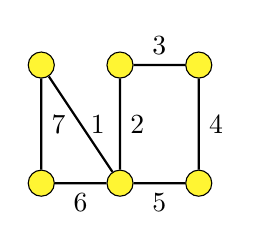
\begin{tikzpicture}
        \node[circle, draw, fill=yellow!80] (a) at (0, 0) {};
        \node[circle, draw, fill=yellow!80] (b) at (1, 0) {};
        \node[circle, draw, fill=yellow!80] (c) at (2, 0) {};
        \node[circle, draw, fill=yellow!80] (d) at (0, -1.5) {};
        \node[circle, draw, fill=yellow!80] (e) at (1, -1.5) {};
        \node[circle, draw, fill=yellow!80] (f) at (2, -1.5) {};
        
        \draw[thick] (a) to node[right] {7} (d)
            (a) to node[right] {1} (e)
            (b) to node[above] {3} (c)
            (c) to node[right] {4} (f)
            (d) to node[below] {6} (e)
            (e) to node[below] {5} (f)
            (b) to node[right] {2} (e);
    \end{tikzpicture}
    \caption{A traversal of the graph that results in an Eulerian cycle.}
\end{figure}
\noindent We take an edge precisely once (but have visited two vertices twice). There is a theorem that states that a connected undirected graph has an Euler cycle if and only if each vertex has an even degree. Therefore, we can test whether a graph has an Eulerian cycle by checking the in-degree of each vertex. So, if we represent the graph as an adjacency matrix, the algorithm is $O(|V|^2)$, while if we use an adjacency list, it is $O(|V| + |E|)$.

Given an undirected graph $G$, we can also ask whether $G$ admits a Hamiltonian cycle. A Hamiltonian cycle is a cycle that visits each vertex precisely once. For example, the graph below has a Hamiltonian cycle shown in red.
\begin{figure}[H]
    \centering
    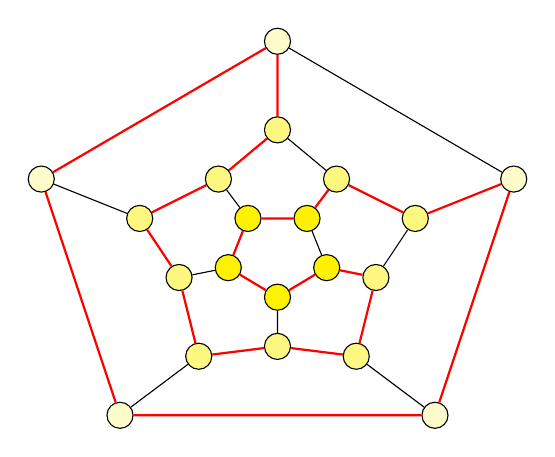
\begin{tikzpicture}
        \node[circle, draw, fill=yellow!20] (a) at (0, -.75) {};
        \node[circle, draw, fill=yellow!20] (b) at (-3, -2.5) {};
        \node[circle, draw, fill=yellow!20] (c) at (3, -2.5) {};
        \node[circle, draw, fill=yellow!20] (d) at (-2, -5.5) {};
        \node[circle, draw, fill=yellow!20] (e) at (2, -5.5) {};
        
        \node[circle, draw, fill=yellow!50] (alt-a) at (0, -1.875) {};
        \node[circle, draw, fill=yellow!50] (alt-b) at (-1.75, -3) {};
        \node[circle, draw, fill=yellow!50] (alt-c) at (1.75, -3) {};
        \node[circle, draw, fill=yellow!50] (alt-d) at (-1, -4.75) {};
        \node[circle, draw, fill=yellow!50] (alt-e) at (1, -4.75) {};
        
        \node[circle, draw, fill=yellow!50] (mid-ab) at (-.75, -2.5) {};
        \node[circle, draw, fill=yellow!50] (mid-ac) at (.75, -2.5) {};
        \node[circle, draw, fill=yellow!50] (mid-bd) at (-1.25, -3.75) {};
        \node[circle, draw, fill=yellow!50] (mid-ce) at (1.25, -3.75) {};
        \node[circle, draw, fill=yellow!50] (mid-de) at (0, -4.625) {};
        
        \node[circle, draw, fill=yellow] (in-e) at (-.375, -3) {};
        \node[circle, draw, fill=yellow] (in-d) at (.375, -3) {};
        \node[circle, draw, fill=yellow] (in-c) at (-.625, -3.625) {};
        \node[circle, draw, fill=yellow] (in-b) at (.625, -3.625) {};
        \node[circle, draw, fill=yellow] (in-a) at (0, -4) {};
        
        \draw[thick, red] (a) to (b)
            (b) to (d)
            (d) to (e)
            (e) to (c)
            (alt-a) to (mid-ab)
            (mid-ab) to (alt-b) 
            (alt-b) to (mid-bd)
            (mid-bd) to (alt-d)
            (alt-d) to (mid-de)
            (mid-de) to (alt-e)
            (alt-e) to (mid-ce)
            (alt-c) to (mid-ac)
            (in-a) to (in-b)
            (in-d) to (in-e)
            (in-e) to (in-c)
            (in-c) to (in-a)
            (a) to (alt-a)
            (c) to (alt-c)
            (mid-ac) to (in-d)
            (mid-ce) to (in-b);
            
        \draw (a) to (c)
            (mid-ac) to (alt-a)
            (e) to (alt-e)
            (mid-ab) to (in-e)
            (mid-bd) to (in-c)
            (b) to (alt-b)
            (d) to (alt-d)
            (mid-ce) to (alt-c)
            (mid-de) to (in-a)
            (in-b) to (in-d);
    \end{tikzpicture}
    \caption{A traversal of the graph that results in a Hamiltonian cycle. The traversal is shown in red.}
\end{figure}
Superficially, the problem seems similar to the Euler cycle problem. However, in an algorithmic sense, they are very different. In fact, nobody has found a polynomial-time algorithm for Hamiltonian cycle. Also, nobody has shown that there does not exist a polynomial-time algorithm to find a Hamiltonian cycle.

One way of finding a Hamiltonian cycle is to generate all the permutations of the vertices. We then check to see if it is a cycle, i.e. the corresponding edges are present. If we have $n$ vertices, then there are $n!$ permutations. For each permutation $\sigma$, it takes $O(n^2)$ to check whether $\sigma$ is a Hamiltonian cycle (assuming $G$ is represented by adjacency lists). In the worst case, to check an edge is present, we have to traverse the adjacency list of length $n-1$, and there are $n$ edges to check. 
% In this case, using an adjacency matrix would have been better since checking whether an edge is present can be done in $O(1)$. 
So, the worst-case number of operations in the brute force approach to find a Hamiltonian cycle using adjacency lists is $O(n^2 n!)$. This is an example of an exponential algorithm.

The table below shows the running time of algorithms with various complexities.
\begin{table}[H]
    \centering
    \scalebox{.95}{
        \begin{tabu}{|c|c|c|c|c|}
            \hline
             & 40 & 50 & 60 & 70 \\
            \hline
            $n$ & $.00003$ secs & $.0004$ secs & $.0005$ secs & $.0006$ secs \\
            \hline
            $n^2$ & $.0009$ secs & $.0016$ secs & $.0025$ secs & $.0036$ secs \\
            \hline
            $n^3$ & $.027$ secs & $.064$ secs & $.125$ secs & $.216$ secs \\
            \hline
            $n^5$ & $24.3$ secs & $1.7$ mins & $5.2$ mins & $13.0$ mins \\
            \tabucline[2pt]{-}
            $2^n$ & $17.9$ mins & $12.7$ days & $35.7$ years & 366 cents \\
            \hline
            $3^n$ & $6.5$ years & 2855 cents & $2 \times 10^8$ cents & $1.3 \times 10^{13}$ cents \\
            \hline
            $n!$ & $8.4 \times 10^{16}$ cents & $2.6 \times 10^{32}$ cents & $9.6 \times 10^{48}$ cents & $2.6 \times 10^{66}$ cents \\
            \hline
        \end{tabu}
    }
    \caption{The running time of algorithms with various complexities (assuming $10^9$ operations per second).}
\end{table}
\noindent Clearly, as $n$ grows, the distinction between polynomial and exponential time algorithms becomes dramatic.

This behaviour still applies even with increases in computing power. Assume that for each time complexity, we have a size $N$ of the largest instance solvable in an hour on a normal computer. The table below shows how the complexity changes as the computer gets faster.
\begin{table}[H]
    \centering
    \begin{tabu}{|c|c|c|c|}
        \hline
         & current & 100 times faster & 1000 times faster \\
        \hline
        $n$ & $N_1$ & $100 \cdot N_1$ & $1000 \cdot N_1$ \\
        \hline
        $n^2$ & $N_2$ & $10 \cdot N_2$ & $31.6 \cdot N_2$ \\
        \hline
        $n^3$ & $N_3$ & $4.64 \cdot N_3$ & $10 \cdot N_3$ \\
        \hline
        $n^5$ & $N_4$ & $2.5 \cdot N_4$ & $3.98 \cdot N_4$ \\
        \tabucline[2pt]{-}
        $2^n$ & $N_5$ & $N_5 + 6.64$ & $N_5 + 9.97$ \\
        \hline
        $3^n$ & $N_6$ & $N_6 + 4.19$ & $N_6 + 6.29$ \\
        \hline
        $n!$ & $N_7$ & $\leq N_7 + 1$ & $\leq N_7 + 1$ \\
        \hline
    \end{tabu}
    \caption{Maximum improvement in computation with increasing computing power.}
\end{table}
\noindent Again, we can see that for polynomial-time algorithms, there is a significant improvement. However, for the exponential algorithms, there is little to no increase.

In summary, exponential-time algorithms are `bad' in general. If we increase the processor speed, there is no significant change in this slow behaviour when the input size is large. On the other hand, polynomial-time algorithms are `good' in general. Often, polynomial-time algorithms require some insight, while exponential-time algorithms are variations on exhaustive search. A problem is polynomial-time solvable if it admits a polynomial-time algorithm.
\newpage

\section{NP-Complete Problems}
There is a set of problems, called NP-complete, for which no polynomial-time algorithm is known. However, if one of them is solvable in polynomial time, then they all are. On the other hand, we also do not know whether they cannot be solved in polynomial time. But, if one of them is not solvable in polynomial time, then they all aren't solvable. 

There are two reasons for a problem to be NP-complete. Either the polynomial time is not sufficient in order to discover a solution, or the solution itself is so large that exponential time is needed to output it. We will only focus on the first case. 

There are many problems that are known to be NP-complete. Moreover, there are some problems have been shown to be undecidable, i.e. there cannot be an algorithm that could solve the problem.

The roadblock problem is a decidable problem that is not solvable in polynomial time. There are two players- $A$ and $B$, along with a network of roads, comprising intersections connected by roads. Each road is coloured either black, blue or green. Some intersections are marked either `$A$ wins' or `$B$ wins'. A player has a fleet of cars at intersections, with at most one per intersection. Player $A$ begins, and subsequently players make moves in turn. They move one of their cars on one or more roads of the same colour. A car may not stop at or pass over an intersection which already has a car. The problem is to decide, for a starting configuration, whether $A$ can win, regardless of what moves $B$ makes.
% TODO: Add Roadblock graph

In summary, there are two classes of problems- polynomial-time solvable problems and intractable problems. We do not know where NP complete problems belong.

A problem is characterised by parameters. Typically, there are infinitely many instances for a given problem. A problem instance is created by giving these parameters values. For example, the Hamiltonian cycle is NP-complete. The problem is:
\begin{itemize}
    \item \textbf{Name}: Hamiltonian Cycle (HC)
    \item \textbf{Instance}: a graph $G$
    \item \textbf{Question}: does $G$ contain a cycle that visits each vertex exactly once?
\end{itemize}
This is an example of a decision problem- for the question, the answer we want is either \texttt{true} or \texttt{false}. So, every instance is either a `yes-instance' or a `no-instance'. 

Another NP-complete problem is the Travelling Salesman Problem, shown below:
\begin{itemize}
    \item \textbf{Name}: Travelling Salesman Decision Problem (TSDP)
    \item \textbf{Instance}: a set of $n$ cities and integer distance $d(i, j)$ between each pair of cities $i, j$, and a target integer $K$
    \item \textbf{Question}: is there a permutation $p_1, p_2, \dots, p_{n-1}, p_n$ of the cities such that
    \[d(p_1, p_2) + d(p_2, p_3) + \dots + d(p_{n-1}, p_n), d(p_n, p_1) \leq K.\]
    That is, can we find a path to travel from one city back to itself (going through all the cities) such that the total distance travelled is less than $K$- such a cycle is called a travelling salesman tour.
\end{itemize}
For example, consider the following graph representation of the cities.
\begin{figure}[H]
    \centering
    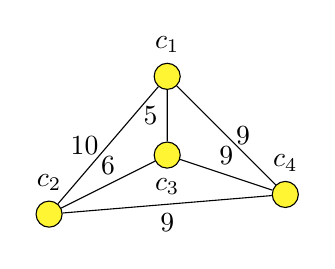
\begin{tikzpicture}
        \node[circle, draw, fill=yellow!80, label={90:$c_1$}] (c1) at (0, 0) {};
        \node[circle, draw, fill=yellow!80, label={90:$c_2$}] (c2) at (-1.5, -1.75) {};
        \node[circle, draw, fill=yellow!80, label={90:$c_4$}] (c4) at (1.5, -1.5) {};
        \node[circle, draw, fill=yellow!80, label={-90:$c_3$}] (c3) at (0, -1) {};
        
        \draw (c1) to node[right] {9} (c4)
            (c1) to node[left] {10} (c2)
            (c2) to node[above] {6} (c3)
            (c4) to node[above] {9} (c3)
            (c1) to node[left] {5} (c3)
            (c2) to node[below] {9} (c4);
    \end{tikzpicture}
\end{figure}
\noindent There is a travelling salesman tour of length 29 when we traverse through the following edges.
\begin{figure}[H]
    \centering
    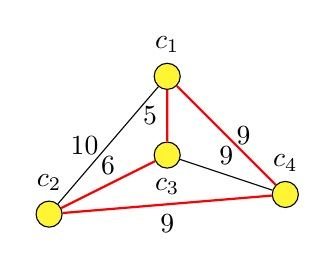
\begin{tikzpicture}
        \node[circle, draw, fill=yellow!80, label={90:$c_1$}] (c1) at (0, 0) {};
        \node[circle, draw, fill=yellow!80, label={90:$c_2$}] (c2) at (-1.5, -1.75) {};
        \node[circle, draw, fill=yellow!80, label={90:$c_4$}] (c4) at (1.5, -1.5) {};
        \node[circle, draw, fill=yellow!80, label={-90:$c_3$}] (c3) at (0, -1) {};
        
        \draw[red, thick] (c1) to node[right, text=black] {9} (c4)
            (c2) to node[below, text=black] {9} (c4)
            (c2) to node[above, text=black] {6} (c3)
            (c1) to node[left, text=black] {5} (c3);
            
        \draw (c1) to node[left] {10} (c2)
            (c4) to node[above] {9} (c3);
    \end{tikzpicture}
\end{figure}
\noindent However, there is no tour of length less than 29. It has been shown that the TSDP is NP-complete.

Another NP-complete problem is the clique problem:
\begin{itemize}
    \item \textbf{Name}: Clique Problem (CP)
    \item \textbf{Instance}: a graph $G$ and a target integer $K$
    \item \textbf{Question}: does $G$ contain a clique of size $K$? That is, does $G$ have a set of $K$ vertices for which there is an edge between all the pairs.
\end{itemize}
For example, the graph below has a clique of size 4, as shown in red.
\begin{figure}[H]
    \centering
    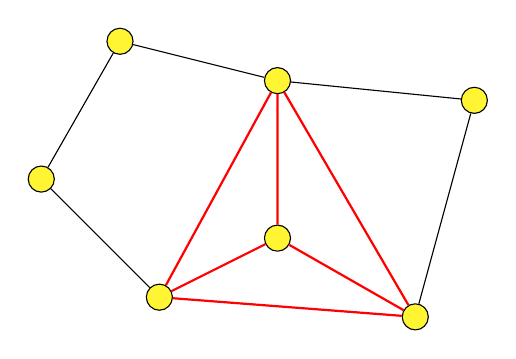
\begin{tikzpicture}
        \node[circle, draw, fill=yellow!80] (a) at (0, 0) {};
        \node[circle, draw, fill=yellow!80] (b) at (-2, .5) {};
        \node[circle, draw, fill=yellow!80] (c) at (2.5, -.25) {};
        \node[circle, draw, fill=yellow!80] (d) at (-3, -1.25) {};
        \node[circle, draw, fill=yellow!80] (e) at (0, -2) {};
        \node[circle, draw, fill=yellow!80] (f) at (-1.5, -2.75) {};
        \node[circle, draw, fill=yellow!80] (g) at (1.75, -3) {};
        
        \draw[red, thick] (a) to (e)
            (a) to (f)
            (a) to (g)
            (f) to (e)
            (e) to (g)
            (f) to (g);
        
        \draw (a) to (b)
            (b) to (d)
            (a) to (c)
            (c) to (g)
            (d) to (f);
    \end{tikzpicture}
\end{figure}
\noindent However, the graph does not have a clique of size 5.

The Graph Colouring Problem is also NP-complete. The problem is:
\begin{itemize}
    \item \textbf{Name}: Graph Colouring Problem (GCP)
    \item \textbf{Instance}: a graph $G$ and a target integer $K$
    \item \textbf{Question}: can one of the $K$ colours be attached to each vertex of $G$ such that the adjacent vertices always have different colours?
\end{itemize}
For example, the graph below can be coloured using 3 colours, as shown below.
\begin{figure}[H]
    \centering
    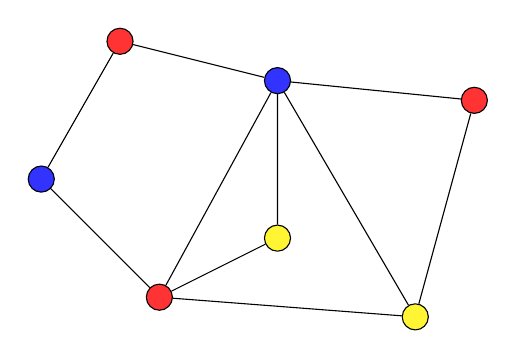
\begin{tikzpicture}
        \node[circle, draw, fill=blue!80] (a) at (0, 0) {};
        \node[circle, draw, fill=red!80] (b) at (-2, .5) {};
        \node[circle, draw, fill=red!80] (c) at (2.5, -.25) {};
        \node[circle, draw, fill=blue!80] (d) at (-3, -1.25) {};
        \node[circle, draw, fill=yellow!80] (e) at (0, -2) {};
        \node[circle, draw, fill=red!80] (f) at (-1.5, -2.75) {};
        \node[circle, draw, fill=yellow!80] (g) at (1.75, -3) {};
        
        \draw (a) to (e)
            (a) to (f)
            (a) to (g)
            (f) to (e)
            (f) to (g)
            (a) to (b)
            (b) to (d)
            (a) to (c)
            (c) to (g)
            (d) to (f);
    \end{tikzpicture}
\end{figure}
\noindent However, there is no colouring using 2 colours.

Finally, we look at the satisfiability problem:
\begin{itemize}
    \item \textbf{Name}: Satisfiability (SAT)
    \item \textbf{Instance}: Boolean expression $B$ in conjunctive normal form (CNF). A CNF is of the form $C_1 \land C_2 \land \dots \land C_n$, where each $C_i$ is a clause. A clause is of the form $l_1 \lor l_2 \lor \dots \lor l_m$, where each $l_j$ is a literal. Finally, a literal is a variable $x$ (which can either be \texttt{true} or \texttt{false}) and its negation $\lnot x$.
    \item \textbf{Question}: Is $B$ satisfiable? That is, can we assign the variables \texttt{true} or \texttt{false} so that the expression $B$ is true.
\end{itemize}
For example, the following boolean expression is in CNF:
\[(x_1 \lor x_2 \lor \lnot x_3) \land (\lnot x_1 \lor x_3 \lor \lnot x_4) \land (\lnot x_2 \lor  x_4) \land (x_2 \lor \lnot x_3 \lor x_4).\]
Also, the expression above is satisfiable if we set $x_1 = \texttt{true}, x_2 = \texttt{false}, x_3 = \texttt{true}, x_4 = \texttt{true}$. The satisfiability problem is NP-complete.

The problems we have looked at have been decision problems- they return \texttt{true} or \texttt{false}. However, we are typically interested in optimisation problem, where we actually have the maximum or the minimum value. For example, the travelling salesman optimisation problem (TSOP) finds the minimum length of a tour. We also have search problems, where we find some appropriate optimal structure. For example, the travelling salesman search problem (TSSP) finds the minimum length tour. 

NP-completeness primarily deals with decision problems, but corresponding to each instance of an optimisation or a search problem is a family of instances of a decision problem by setting the `target' values. Almost invariably, an optimisation or a search problem can be solved in polynomial time if and only if the corresponding decision problem can.
\newpage

\section{P and NP}
The class P is the set of all decision problems that can be solved in polynomial time. There are many problems in P, e.g.
\begin{itemize}
    \item Is there a path of length $\leq K$ from vertex $u$ to vertex $v$ in a graph $G$?
    \item Is there a spanning tree of weight $\leq K$ in a graph $G$?
    \item Is a graph $G$ bipartile?
    \item Is a graph $G$ connected?
    \item Does a directed graph $D$ contain a cycle?
    \item Does a text $t$ contain an occurrence of a string $s$?
    \item For two strings $s$ and $t$, is their distance $d(s, t) \leq K$?
\end{itemize}
P is often extended to include search and optimisation problems.

The class NP is the set of decision problems that can be solved in non-deterministic polynomial time. A non-deterministic algorithm can make non-deterministic (random) choices, so it can give different answers depending on when we run it. Hence, it is apparently more powerful than a normal deterministic algorithm.

Clearly, P is contained within NP- a deterministic algorithm is just a special case of a non-deterministic one. But, the containment may not be strict. Currently, there is no problem known to be in NP and not in P.

A non-deterministic algorithm (NDA) have an extra operation- they can make a non-deterministic choice. A NDA has many possible executions depending on which values were chosen during the process. We say that NDA `solves' a decision problem $\Pi$ if for a yes-instance $I$ of $\Pi$, there is some execution that returns \texttt{true}, and for any no-instance $I$ of $\Pi$, there is no execution that returns \texttt{true}. Moreover, the NDA `solves' a decision problem $\Pi$ in polynomial time if for a yes-instance $I$ of $\Pi$, there is some execution that returns \texttt{true} which uses a number of steps bounded by a polynomial in the input, and for a no-instance, there is no execution that returns \texttt{true}.

Clearly, NDAs are not useful in practice since they do not always return the right answer. However, they are a useful mathematical concept for defining the classes of NP and NP-complete problems.

We will now provide a NDA that `solves' the graph colouring problem.
\lstinputlisting[language=pseudocode]{src/graphColouring.psc}
In line 4, we make a non-deterministic choice for the colour of a vertex from the set of $k$ colours. We then check whether the coloured graph satisfies the graph colouring problem. The operations take polynomial time for every execution of the algorithm.

In general, a NDA can be viewed as having a guessing stage (which is non-deterministic), and a checking stage (which is determinstic). The guessing stage is usually $O(n)$. So, for a problem to be in NP, we need the checking stage to run in polynomial time.
\newpage

\section{Polynomial-time reductions}
A polynomial-time reduction (PTR) is a mapping $f$ from a decision problem $\Pi_1$ to a decision problem $\Pi_2$ such that for every instance $I_1$ of $\Pi_1$, the instance $f(I_1)$ of $\Pi_2$ can be constructed in polynomial time. Moreover, $f(I_1)$ is a yes-instance of $\Pi_2$ if and only if $I_1$ is a yes-instance of $\Pi_1$. We denote this as $\Pi_1 \varpropto \Pi_2$.

Polynomial-time reductions are transitive. That is, if we have decision problems $\Pi_1, \Pi_2, \Pi_3$ such that $\Pi_1 \varpropto \Pi_2$ and $\Pi_2 \varpropto \Pi_3$, then $\Pi_1 \varpropto \Pi_3$. By definition, there exist PTRs $f$ from $\Pi_1$ to $\Pi_2$ and $g$ from $\Pi_2$ to $\Pi_3$. Now, for any instance $I_1$ of $\Pi_1$, we can create an instance $f(I_1)$ of $\Pi_2$ in polynomial time. By definition, $f(I_1)$ has the same answer as $I_1$. Moreover, $g$ is a PTR as well, so $g(f(I_1))$ is an instance of $\Pi_3$ that we can construct from $f(I_1)$ in polynomial time. By definition, $g(f(I_1))$ has the same answer as $f(I_1)$. Therefore, the composition $g \circ f$ is a polynomial time reduction from $\Pi_1$ to $\Pi_3$ since $(g \circ f)(I_1)$ has the same answer as $I_1$.

If we have $\Pi_1 \varpropto \Pi_2$ and $\Pi_2 \in P$, then $\Pi_1 \in P$ as well. To solve an instance of $\Pi_1$, we can reduce it to an instance of $\Pi_2$ in polynomial-time. Then, we can solve $\Pi_2$ in polynomial-time and return the result. The entire process takes polynomial time, so $\Pi_1 \in P$. 

Roughly speaking, $\Pi_1 \varpropto \Pi_2$ means that $\Pi_1$ is `no harder' than $\Pi_2$. That is, if we can solve $\Pi_2$, then we can solve $\Pi_1$ without much more effort- we just need to perform a polynomial time reduction. It is also possible that $\Pi_2$ is harder to solve than $\Pi_1$. We may only map the instances of $\Pi_1$ to those in $\Pi_2$ that are `easy' to solve.

We can reduce the Hamiltonian cycle problem to the travelling salesman problem. For instance, assume that we are given the following instance of the Hamiltonian cycle problem.
\begin{figure}[H]
    \centering
    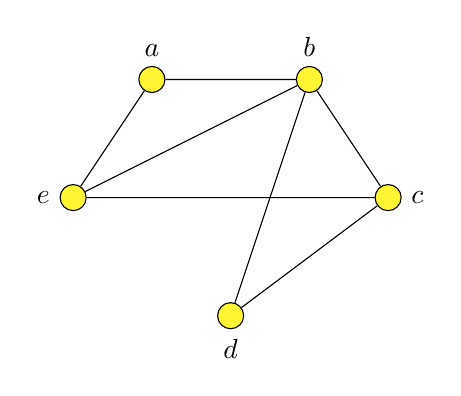
\begin{tikzpicture}
        \node[circle, draw, fill=yellow!80, label={90:$a$}] (a1) at (-1, 1) {};
        \node[circle, draw, fill=yellow!80, label={90:$b$}] (b1) at (1, 1) {};
        \node[circle, draw, fill=yellow!80, label={0:$c$}] (c1) at (2, -.5) {};
        \node[circle, draw, fill=yellow!80, label={-90:$d$}] (d1) at (0, -2) {};
        \node[circle, draw, fill=yellow!80, label={180:$e$}] (e1) at (-2, -.5) {};
        
        \draw (a1) to (b1)
            (b1) to (c1)
            (c1) to (d1)
            (a1) to (e1)
            (b1) to (e1)
            (e1) to (c1)
            (b1) to (d1);
    \end{tikzpicture}
    \caption{An instance of the Hamiltonian Cycle problem.}
\end{figure}
\noindent We will construct a TSDP corresponding to this graph. So, let the vertices be the cities in the problem. Moreover, for two cities $x, y$, we set $d(x, y) = 1$ if there is an edge $\{x, y\}$ in the graph above, and $d(x, y) = 2$ otherwise. Then, we can set $K$ to be the number of edges. This gives us the following graph.
\begin{figure}[H]
    \centering
    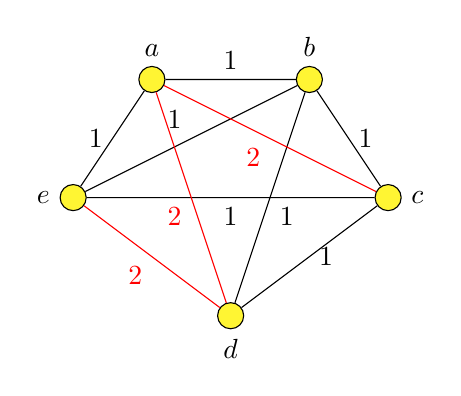
\begin{tikzpicture}
        \node[circle, draw, fill=yellow!80, label={90:$a$}] (a2) at (5, 1) {};
        \node[circle, draw, fill=yellow!80, label={90:$b$}] (b2) at (7, 1) {};
        \node[circle, draw, fill=yellow!80, label={0:$c$}] (c2) at (8, -.5) {};
        \node[circle, draw, fill=yellow!80, label={-90:$d$}] (d2) at (6, -2) {};
        \node[circle, draw, fill=yellow!80, label={180:$e$}] (e2) at (4, -.5) {};
        
        \draw (a2) to node[above] {1} (b2)
            (b2) to node[right] {1} (c2)
            (c2) to node[right] {1} (d2)
            (a2) to node[left] {1} (e2)
            (b2) to node[above left] {1} (e2)
            (e2) to node[below] {1} (c2)
            (b2) to node[below right] {1} (d2);
        \draw[red] (a2) to node[below left] {2} (d2)
            (e2) to node[below left] {2} (d2)
            (a2) to node[below left] {2} (c2);
    \end{tikzpicture}
    \caption{An instance of the Travelling Salesman Problem}
\end{figure}
\noindent All these operations can be performed in polynomial-time. Moreover, the graph has a travelling salesman tour of length $\leq K$ if and only if the original graph has a Hamiltonian cycle. The tour includes $|E|$ edges, so we cannot take any edges with weight 2. So, if the travelling salesman problem is in P, then the Hamiltonian cycle problem is in P as well.

We now define NP-completeness. We say that a decision problem $\Pi$ is NP-complete if $\Pi$ is in NP, and for every problem $\Pi'$ in NP, the problem $\Pi'$ reduces to $\Pi$ in polynomial-time. If $\Pi$ is NP-complete and $\Pi$ is in P as well, then we have P = NP. Every problem in NP can be solved in polynomial time by reduction to $\Pi$. Supposing P $\neq$ NP, if $\Pi$ is NP-complete, then $\Pi$ is not in P.

To prove that a problem is NP-complete, it is not feasible to describe a reduction from every problem in NP. However, if we know that a problem $\Pi_1$ is NP-complete, then to show that another problem $\Pi_2$ is NP-complete, we need to show that $\Pi_2$ is in NP and that there exists a polynomial-time reduction from $\Pi_1$ to $\Pi_2$. Since $\Pi_1$ is NP-complete, we know that for any problem $\Pi$ in NP, we have $\Pi \varpropto \Pi_1$. We also know that $\Pi_1 \varpropto \Pi_2$. Since $\varpropto$ is transitive, it follows that $\Pi \varpropto \Pi_2$. Therefore, $\Pi_2$ is NP-complete.

We know that the satisfiability problem (SAT) is NP-complete. The proof consists of a generic polynomial-time reduction to SAT from an abstract definition of a general problem in the class NP. The generic reduction could be instantiated to give an actual reduction for each individual NP problem. So, to prove that a decision problem $\Pi$ is NP-complete, we need to show that $\Pi$ is in NP and that there is some polynomial-time that reduces SAT to $\Pi$.

We will use this technique to show that the Clique problem (CP) is NP-complete. To prove CP is NP-complete, we show that CP is in NP and that there exists a polynomial-time reduction from SAT to CP. The following is an NDA that solves the CP.
\lstinputlisting[language=pseudocode]{src/clique.psc}
We can guess the solution in $O(K)$ time, and check in $O(K^2)$. Therefore, the problem is in NP.

Next, we show that there is a polynomial-time reduction from SAT to CP. So, assume that we are given an instance $B$ of SAT. We construct an instance $(G, K)$ of CP. We set $K$ to be the number of clauses of $B$. The vertices of $G$ are $(l, C)$, where $l$ is a literal in clause $C$. We add an edge $\{(l, C), (m, D)\}$ if $l \neq \lnot m$ and $C \neq D$. That is, we add an edge if distinct literals from different clauses can be satisfied simultaneously. This is a polynomial-time algorithm since the construction takes $O(n^2)$- in the worst case, we need to compare every literal with every other literal when constructing the edges.

Now, if $B$ has a satisfying assignment, then if we choose a \texttt{true} literal in each clause, the corresponding vertices form a clique of size $K$ in $G$. On the other hand, if $G$ has a clique of size $K$, then assigning each literal associated with a vertex in the clique to be \texttt{true} yields a satisfying assignment for $B$. 

We only have edges between literals in distinct clauses, so if we have a clique of size $K$, then it must include precisely one literal from each clause. Moreover, we can satisfy all the literals in the clique simultaneously, since a clause is a disjunction of the literals and we can satisfy one of the literals. Moreover, this satisfies $B$ since $B$ is the conjunction of the clauses, and we satisfy all the clauses.

We will illustrate this with an example. Assume that we are given the following CNF.
\[({\color{orange} x_1} \lor {\color{orange} x_2} \lor {\color{orange} \lnot x_3}) \land ({\color{red} \lnot x_1} \lor {\color{red} x_3} \lor {\color{red} \lnot x_4}) \land ({\color{blue} \lnot x_2} \lor {\color{blue} x_4}) \land ({\color{green} x_2} \lor {\color{green} \lnot x_3} \lor {\color{green} x_4})\]
There are 4 vertices, so $K = 4$. The graph $G$ consists of $(l, C)$, where $l$ is a literal in clause $C$. We can join them if they are from different clauses and can be satisfied together. So, this gives us the following graph.
\begin{figure}[H]
    \centering
    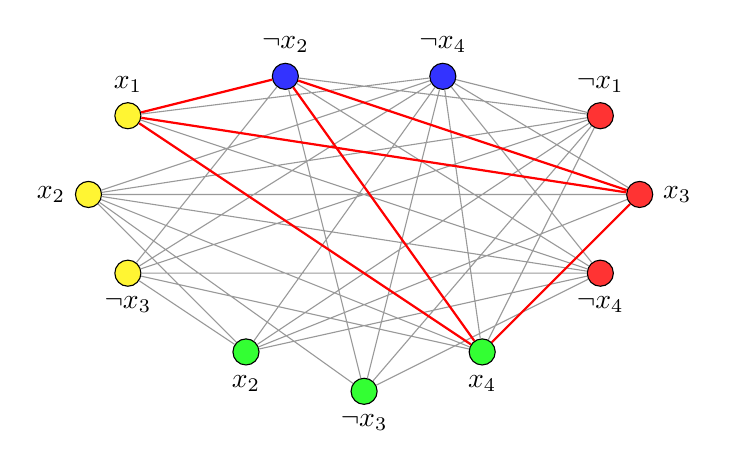
\begin{tikzpicture}
        \node[circle, draw, fill=yellow!80, label={90:$x_1$}] (x1) at (-3, 0) {};
        \node[circle, draw, fill=yellow!80, label={180:$x_2$}] (x2) at (-3.5, -1) {};
        \node[circle, draw, fill=yellow!80, label={-90:$\lnot x_3$}] (x3) at (-3, -2) {};
        
        \node[circle, draw, fill=red!80, label={90:$\lnot x_1$}] (y1) at (3, 0) {};
        \node[circle, draw, fill=red!80, label={0:$x_3$}] (y3) at (3.5, -1) {};
        \node[circle, draw, fill=red!80, label={-90:$\lnot x_4$}] (y4) at (3, -2) {};
        
        \node[circle, draw, fill=blue!80, label={90:$\lnot x_2$}] (z2) at (-1, .5) {};
        \node[circle, draw, fill=blue!80, label={90:$\lnot x_4$}] (z4) at (1, .5) {};
        
        \node[circle, draw, fill=green!80, label={-90:$x_2$}] (w2) at (-1.5, -3) {};
        \node[circle, draw, fill=green!80, label={-90:$\lnot x_3$}] (w3) at (0, -3.5) {};
        \node[circle, draw, fill=green!80, label={-90:$x_4$}] (w4) at (1.5, -3) {};
        
        \draw[gray!80] (x1) to (y4)
            (x1) to (z4)
            (x1) to (w4)
            
            (x2) to (y1)
            (x2) to (y3)
            (x2) to (y4)
            (x2) to (z4)
            (x2) to (w3)
            (x2) to (w2)
            (x2) to (w4)
            
            (x3) to (y1)
            (x3) to (y4)
            (x3) to (z2)
            (x3) to (z4)
            (x3) to (w2)
            (x3) to (w4)
            
            (y1) to (z2)
            (y1) to (z4)
            (y1) to (w2)
            (y1) to (w3)
            (y1) to (w4)
            
            (y3) to (z2)
            (y3) to (z4)
            (y3) to (w2)
            (y3) to (w4)
            
            (y4) to (z2)
            (y4) to (z4)
            (y4) to (w2)
            (y4) to (w3)
            
            (z2) to (w3)
            (z2) to (w4)
            
            (z4) to (w2)
            (z4) to (w3)
            (z4) to (w4);
        
        \draw[thick, red] (x1) to (y3)
            (x1) to (z2)
            (x1) to (w4)
            (y3) to (z2)
            (y3) to (w4)
            (z2) to (w4);
    \end{tikzpicture}
\end{figure}
\noindent Highlighted in red is the clique of size 4. So, setting $x_1 = \texttt{true}, \lnot x_2 = \texttt{true}, x_3 = \texttt{true}, x_4 = \texttt{true}$ satisfies $B$.

\subsection{Problem Restrictions}
A restriction of a problem consists of a subset of the instances of the original problem. If a restriction of a given decision problem $\Pi$ is NP-complete, then so is $\Pi$. However, given an NP-complete problem $\Pi$, a restriction of $\Pi$ might be NP-complete. 

For example, a clique restricted to cubic graphs is in P. By definition, a cubic graph is a graph in which every vertex belongs to 3 edges. A largest clique has size at most 4, so exhaustive search is $O(n^4)$. On the other hand, if we restrict graph colouring to cubic graphs, the problem remains NP-complete.

The $K$-colouring problem is a restriction of GCP for a fixed number $K$ of colours. A 2-colouring problem is in P, since it reduces to checking the graph is bipartile. On the other hand, 3-colouring is NP-complete. 

Similarly, $K$-SAT is a restriction of SAT in which every clause contains exactly $K$ literals. 2-SAT is in P, but 3-SAT is NP-complete. We can prove this by showing that SAT can be reduced to 3-SAT. So, assume we are given an instance $B$ of SAT. We will construct an instance $B'$ of 3-SAT. For each clause $C$ of $B$, we construct a number of clauses of $B'$, as shown below:
\begin{itemize}
    \item If $C = l_1$, we introduce 2 addition variables $x_1$ and $x_2$ and add the clauses: $(l_1 \lor x_1 \lor x_2), (l_1 \lor x_1 \lor \lnot x_2), (l_1 \lor \lnot x_1 \lor x_2)$ and $(l_1 \lor \lnot x_1 \lor \lnot x_2)$ to $B'$. The conjunction of these clauses can be satisfied if and only if $l_1$ is \texttt{true}.
    \item If $C = (l_1 \lor l_2)$, then we introduce a variable $y$ and add the clauses $(l_1 \lor l_2 \lor \lnot y)$ and $(l_1 \lor l_2 \lor \lnot y)$. The conjunction of these clauses can be satisfied if and only if $l_1 \lor l_2 = \texttt{true}$.
    \item If $C = (l_1 \lor l_2 \lor l_3)$, then we can just add the clause to $B'$.
    \item If $C = (l_1 \lor \dots \lor l_k)$ (for $k > 3$), then we introduce $k-3$ additional variables $z_1, \dots, z_{k-3}$ and add the clauses: $(l_1 \lor l_2 \lor z_1), (\lnot z_1 \lor l_3 \lor z_2), (\lnot z_2 \lor l_4 \lor z_3), \dots, (\lnot z_{k-4} \lor l_{k-2} \lor z_{k-3}), (\lnot z_{k-3} \lor l_{k-1} \lor l_k)$. Again, all the clauses hold if and only if $C$ holds.
\end{itemize}

If we have a problem that is NP-complete, we can try restricting a problem if only a particular class of problems are of interest, given that the restriction is in P. We can seek an exponential-time algorithm that improves on exhaustive search. Moreover, for an optimisation problem, we could settle for an approximation algorithm that runs in polynomial time, especially if it gives a provably good result (within some factor of the optimal solution). For a decision problem, we can settle for a probabilistic algorithm that gives the correct answer with high probability.


\end{document}
